\section{推前测度}
\label{sec:measure-pushforward}

可测映射保证输出端的集合问题在输入端有意义。若输入端还配有测度，就可以回答“输出落在$B$中的质量有多少”：把会被送进$B$的输入全部找出来，累计它们的质量。本节用这一想法定义推前测度，核对它的可加性、复合与总量的变化，再用多对一映射和坐标投影计算具体的推前。整节只用到原像与测度的取值；推前测度下的积分换元公式在第~\ref{sec:integral-change-of-variables}节建立。

\subsection{推前测度的定义与性质}
\label{sec:measure-pushforward-def}

\paragraph{用原像累计质量}
设$T:(X,\mathcal A)\to(Y,\mathcal B)$可测，$\mu$是$(X,\mathcal A)$上的测度。对$B\in\mathcal B$，输出落在$B$中的输入恰是$T^{-1}(B)$，它可测，于是可以取它的质量作为$B$的质量。

\begin{definition}[推前测度]
\label{def:measure-pushforward}
设$T:(X,\mathcal A)\to(Y,\mathcal B)$可测，$\mu$是$(X,\mathcal A)$上的测度。令
\[
 (T_\#\mu)(B)=\mu\bigl(T^{-1}(B)\bigr),\qquad B\in\mathcal B,
\]
称$T_\#\mu$为$\mu$在$T$下的\term{推前测度}（pushforward measure）。
\end{definition}

\begin{theorem}[推前测度的基本性质]
\label{thm:measure-pushforward-properties}
在上述记号下：
\begin{enumerate}
 \item $T_\#\mu$是$(Y,\mathcal B)$上的测度，且$(T_\#\mu)(Y)=\mu(X)$；特别地，有限测度推前后仍有限，概率测度推前后仍是概率测度。
 \item 若$S:(Y,\mathcal B)\to(Z,\mathcal C)$也可测，则$(S\circ T)_\#\mu=S_\#(T_\#\mu)$。
\end{enumerate}
\end{theorem}

\begin{proof}
对第1条，$T^{-1}(\varnothing)=\varnothing$给出空集为零。若$B_n\in\mathcal B$两两不交，则它们的原像也两两不交：一个$x$若同时属于$T^{-1}(B_n)$与$T^{-1}(B_m)$，$T(x)$就同时属于$B_n$与$B_m$。由$T^{-1}(\bigcup_nB_n)=\bigcup_nT^{-1}(B_n)$和$\mu$的可数可加性，
\[
 (T_\#\mu)\Bigl(\bigcup_nB_n\Bigr)=\mu\Bigl(\bigcup_nT^{-1}(B_n)\Bigr)=\sum_n\mu\bigl(T^{-1}(B_n)\bigr)=\sum_n(T_\#\mu)(B_n).
\]
总量由$T^{-1}(Y)=X$得到。对第2条，$S\circ T$可测（第~\ref{sec:measure-preimage-criterion}小节），且对$C\in\mathcal C$，$(S\circ T)^{-1}(C)=T^{-1}(S^{-1}(C))$，于是$((S\circ T)_\#\mu)(C)=\mu(T^{-1}(S^{-1}(C)))=(T_\#\mu)(S^{-1}(C))=(S_\#(T_\#\mu))(C)$。
\end{proof}

第2条说明，分两步传递质量与一步传递质量的结果相同；这使我们可以把复杂的映射拆成简单映射逐步计算推前。

\paragraph{保持测度的映射}
当$T$把空间映到自身时，可以问质量分布是否在传递后保持不变。若可测映射$T:(X,\mathcal A)\to(X,\mathcal A)$满足$T_\#\mu=\mu$，即$\mu(T^{-1}(A))=\mu(A)$对一切$A\in\mathcal A$成立，称$T$\term{保持测度}（measure-preserving）。在$X=\{0,1,\dots,n-1\}$上取计数测度与循环移位$T(k)=k+1\bmod n$，$T$是双射，$T^{-1}(A)$与$A$元素个数相同，所以$T$保持计数测度。在实轴上，平移$T(x)=x+t$满足$T^{-1}(B)=B-t$，由Lebesgue测度的平移不变性，$\lambda(B-t)=\lambda(B)$，平移保持$\lambda$。

伸缩则改变长度。令$T(x)=2x$。区间$(a,b]$的原像是$T^{-1}((a,b])=(a/2,b/2]$，所以$(T_\#\lambda)((a,b])=(b-a)/2$。两个测度$T_\#\lambda$与$\tfrac12\lambda$在$\pi$系统$\{\varnothing\}\cup\{(a,b]\}$上一致，且在覆盖片$(-n,n]$上都取有限值$n$，由定理~\ref{thm:measure-uniqueness}，$T_\#\lambda=\tfrac12\lambda$。把实轴拉长一倍，同一个输出区间只收集到原来一半长度的输入。

\paragraph{$\sigma$有限性一般不保持}
总量在推前下不变，因此有限与概率的性质保持；$\sigma$有限性却可能丢失，因为推前可以把无限多片有限质量集中到一个点。在$\mathbb N$上取计数测度$\mu$，它是$\sigma$有限的。令$T$把$\mathbb N$映到单点集$Y=\{y\}$（取$\mathcal P(Y)$），则$(T_\#\mu)(\{y\})=\mu(\mathbb N)=+\infty$；$Y$的可测子集只有$\varnothing$与$\{y\}$，无法写成有限质量集合的可数并，$T_\#\mu$不是$\sigma$有限的。需要唯一性定理或后面的分解定理时，推前测度的$\sigma$有限性必须单独核对。

\subsection{合并与投影产生的测度}
\label{sec:measure-merge-projection}

\paragraph{多对一映射合并质量}
推前不要求$T$是单射。若有几个输入被送到同一个输出，它们的质量在输出处相加。设$X=\{1,2,3,4\}$上的测度$\mu$给四个点分别赋权$0.1,0.2,0.3,0.4$，$T(1)=T(3)=a$，$T(2)=T(4)=b$。则$T^{-1}(\{a\})=\{1,3\}$，$T^{-1}(\{b\})=\{2,4\}$，
\[
 T_\#\mu=0.4\,\delta_a+0.6\,\delta_b.
\]
图~\ref{fig:measure-pushforward-merge}(a)画出了这一过程：每个输出点收集其全部原像的权重，原来的四个点在输出端只剩两个，总量仍为$1$。

推前还可以把分布在区间上的质量合并成点质量。令$\mu=\lambda|_{[0,1]}$，$T$为取常值$c$的映射。对Borel集$B$，若$c\in B$，则$T^{-1}(B)=\mathbb R$，否则$T^{-1}(B)=\varnothing$，所以$(T_\#\mu)(B)=\mathbf 1_B(c)\cdot\lambda([0,1])$，即$T_\#\mu=\delta_c$。每个单点在$\mu$下质量为零，推前后却得到质量为$1$的点；区别在于原像$T^{-1}(\{c\})$是整个区间，而不是单点。若改用$T(x)=\lfloor2x\rfloor$，原像$T^{-1}(\{0\})\cap[0,1]=[0,\tfrac12)$、$T^{-1}(\{1\})\cap[0,1]=[\tfrac12,1)$、$T^{-1}(\{2\})\cap[0,1]=\{1\}$，得$T_\#\mu=\tfrac12\delta_0+\tfrac12\delta_1$，见图~\ref{fig:measure-pushforward-merge}(b)。

\begin{figure}[!htbp]
  \centering
  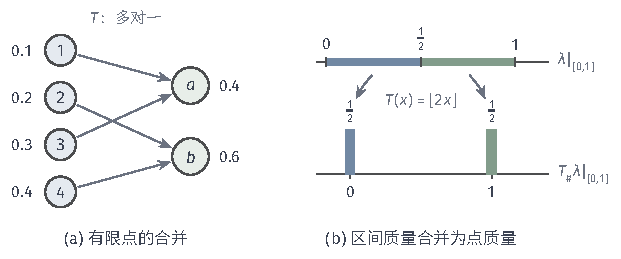
\includegraphics[width=105.1mm]{figures/02-abstract-mathematics/01-metric-and-measure/tikz/c2-pushforward-merge/figure.pdf}
  \caption{推前测度累计原像的质量。(a)四个带权点经多对一映射送到$a,b$两点，$a$收集点$1,3$的权重$0.1+0.3=0.4$，$b$收集点$2,4$的权重$0.2+0.4=0.6$；(b)$[0,1]$上的长度测度经$T(x)=\lfloor2x\rfloor$推前，原像$[0,\tfrac12)$与$[\tfrac12,1)$的长度分别汇集为点$0$和点$1$处的质量$\tfrac12$，单点$\{1\}$的长度为零，不贡献质量。}
  \label{fig:measure-pushforward-merge}
\end{figure}

\paragraph{坐标投影与边缘测度}
多元问题中最常见的多对一映射是坐标投影。设$\mu$是$\mathcal B(\mathbb R^d)$上的测度，$1\le k<d$，$\pi(\bm x)=(x_1,\dots,x_k)$。$\pi$连续，因而Borel可测，且对$B\in\mathcal B(\mathbb R^k)$有$\pi^{-1}(B)=B\times\mathbb R^{d-k}$，所以
\[
 (\pi_\#\mu)(B)=\mu\bigl(B\times\mathbb R^{d-k}\bigr).
\]
$\pi_\#\mu$称为$\mu$在前$k$个坐标上的\term{边缘测度}（marginal measure）：它忽略后$d-k$个坐标，只记录前$k$个坐标落在何处。卷一用联合分布对其余变量求和或积分得到边缘分布（可参考\BookChapterRef{chap:random-vectors}{卷一“随机向量与联合分布”章}），这里的定义只用集合原像，对离散与连续情形同样适用。

\begin{example}[点质量与单位正方形的投影]
\label{ex:measure-projection-marginal}
在$\mathbb R^2$上取$\mu=0.2\,\delta_{(0,0)}+0.3\,\delta_{(0,1)}+0.5\,\delta_{(1,1)}$。第一坐标的投影$\pi_1$把$(0,0)$与$(0,1)$都送到$0$，所以$(\pi_1)_\#\mu=0.5\,\delta_0+0.5\,\delta_1$；第二坐标的投影把$(0,1)$与$(1,1)$都送到$1$，所以$(\pi_2)_\#\mu=0.2\,\delta_0+0.8\,\delta_1$。

再取$\nu=\lambda_2|_{[0,1]^2}$。对$B=(a,b]$，$\pi_1^{-1}(B)\cap[0,1]^2=\bigl((a,b]\cap[0,1]\bigr)\times[0,1]$是一个矩形，面积等于$\lambda((a,b]\cap[0,1])$乘以$1$。于是$(\pi_1)_\#\nu$与$\lambda|_{[0,1]}$在全部$(a,b]$上一致，总量都为$1$，由定理~\ref{thm:measure-uniqueness}，二者在$\mathcal B(\mathbb R)$上相等。图~\ref{fig:measure-projection-marginal}画出了两种情形。
\end{example}

\begin{figure}[!htbp]
  \centering
  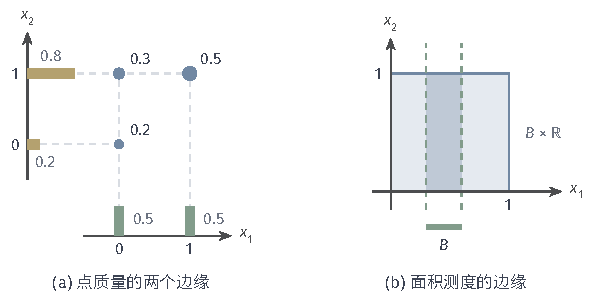
\includegraphics[width=100.9mm]{figures/02-abstract-mathematics/01-metric-and-measure/tikz/c2-projection-marginal/figure.pdf}
  \caption{坐标投影产生的边缘测度。(a)平面上三个点质量$0.2,0.3,0.5$，向横轴投影得到$0.5\delta_0+0.5\delta_1$，向纵轴投影得到$0.2\delta_0+0.8\delta_1$；(b)单位正方形上的面积测度，横轴区间$B$的边缘质量等于竖条$B\times\mathbb R$与正方形之交的面积，结果是$[0,1]$上的长度。}
  \label{fig:measure-projection-marginal}
\end{figure}

边缘测度的总量与原测度相同，但$\sigma$有限性同样可能丢失：对整个平面上的$\lambda_2$，任一非退化区间$B$都有$(\pi_1)_\#\lambda_2(B)=\lambda_2(B\times\mathbb R)=+\infty$，输出测度在每个非空开区间上都无限。对坐标积分把联合测度的计算化为边缘上的计算，以及一般推前测度下的积分公式，都在第~\ref{chap:integration}章建立；边缘测度何时有密度、密度怎样计算，在第~\ref{chap:densities-change-of-measure}章讨论。这里不预设输出测度一定有密度：上面的点质量例子中，边缘测度就是离散的。
